\documentclass[12pt,a4paper]{article}

\usepackage[utf8]{inputenc}
\usepackage[T1]{fontenc}
\usepackage[english]{babel}
\usepackage{amsmath}
\usepackage{amsfonts}
\usepackage{ae}
\usepackage{units}
\usepackage{icomma}
\usepackage{color}
\usepackage{graphicx}
\usepackage{bbm}
\usepackage{upgreek}
\usepackage{amsthm}
\usepackage{fullpage}
\usepackage{mathtools}
\usepackage{psfrag}
\usepackage{caption}
\usepackage{fancyhdr}
\usepackage[table]{xcolor}
\usepackage{longtable}
\usepackage{hyperref}
\usepackage{tocloft}
\usepackage{epstopdf}
\renewcommand{\cftdotsep}{\cftnodots}
\setlength\parindent{0pt}

\begin{document}

\title{IM2601 Solid State Physics \\
Lab exercise 2: Superconductivity}
\author{Karl Amundsson karlam@kth.se\\
Alexander Bielik abielik@kth.se\\
Hannes Lindström halinds@kth.se}
\date{\today}
\maketitle
\thispagestyle{empty}

\newpage

\tableofcontents
\thispagestyle{empty}

\newpage
\setcounter{page}{1}

\section{Introduction}

Superconductors are materials that below certain critical temperatures $T_c$, magnetic fields and current densities share a number of remarkable properties, including lacking electrical resistance and internal magnetic fields \cite{kittel}. These materials are furthermore divided into two different types. In type-II superconductors, vortices can form in which the magnetic field is not zero given an external field strength above a critical value, which is a phenomenon that does not occur with type-I superconductors. \\

The applications of superconductors are numerous, mainly because of their potential of leading currents with practically no energy losses. A major complication that arises and greatly increases the costs is the need for extremely low temperatures to make the resistance drop to zero. For this reason, superconductors that can operate at relatively high temperatures are currently the subject of much research. Above 77 K, liquid nitrogen can be used instead of the much more expensive liquid helium and the cooling effect required is by itself greatly reduced compared to superconductors requiring a few K. \\

In this lab exercise \cite{lab_PM}, a sample of the high temperature superconductor YBa$_2$Cu$_3$O$_{7-\updelta}$ (YBCO) is cooled from room temperature to become superconductive and then reheated. The electrical resistance is measured as a function of the temperature for this process.

\section{Experimental procedure}

The experimental setup consisted of a measurement adapter with power supply, a module containing the YBCO sample encased in aluminium, a packaging box, liquid nitrogen and a computer. The basic measurement setup is displayed in figure \ref{setup}.

\begin{figure}[ht!]
\centering
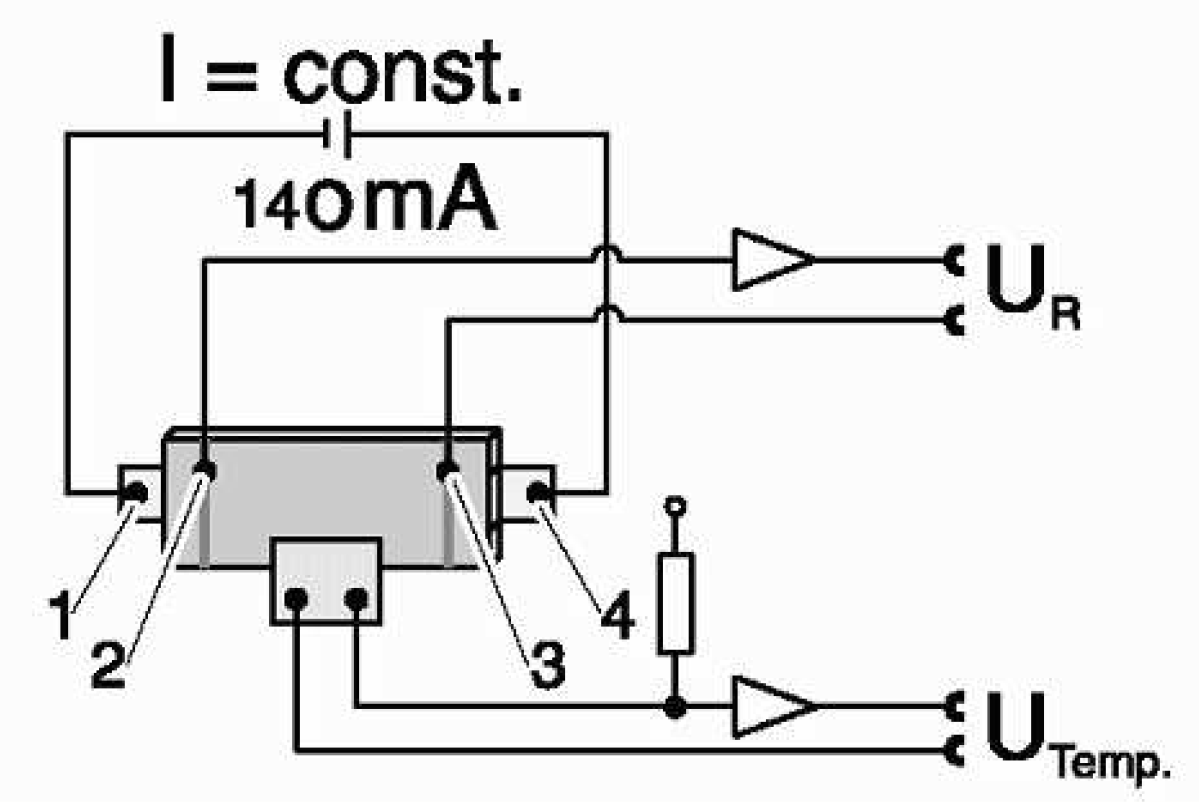
\includegraphics[scale=0.25]{setup.png}
\caption{Measurement setup, taken from \cite{lab_PM}}
\label{setup}
\end{figure}

The module was connected to the adapter through the contacts displayed and placed in the packaging. The adapter was connected to the power supply and the computer running the software CASSY Lab via USB. The measurement was started and liquid nitrogen was poured onto the module. Once the temperature had been below $T_c$ for a while, the module was removed and placed on the side. After the temperature had gone above $T_c$ again for some time, the measurement was completed and data was collected for post-processing. The data points were taken in intervals of 5 s and the total process lasted about 31 minutes. \\

The measurement method used in the lab exercise with contacts 1, 2, 3 and 4 is known as the four-point technique. A current of 140 mA was sent through the YBCO sample by contacts 1 and 4, allowing the voltage drop $U_R$ to be measured using contacts 2 and 3. The reason that this technique is appropriate in this case is that the resistance induced by contacts 1 and 4 does not influence $U_R$ and thus allows for very small resistances to be measured with no interference. In the measurement adapter, $U_R$ was amplified with some factor, resulting in the output voltage $U_A$ that has here been considered. \\

Using the two remaining contacts, the voltage $U_{temp}$ was measured through an iridium resistor. Since the resistance of the resistor has a known temperature dependence, this allowed for the temperature $T$ of the YBCO sample to be determined.
\section{Measurement results}

In figure \ref{results}, the measured output voltage $U_A$ is plotted against the temperature of the sample. Since the zero level of the voltage was not configured beforehand, the voltage data collected have been subtracted by the lowest value.

\begin{figure}[ht!]
\centering
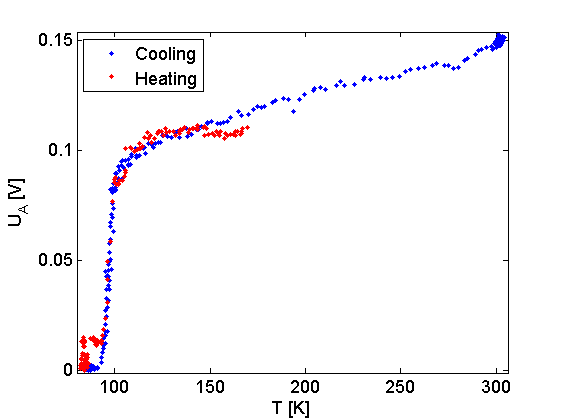
\includegraphics [scale=0.75]{results.png}
\caption{Output voltage $U_A$ to temperature $T$ of the YBCO sample}
\label{results}
\end{figure}

\section{Discussion of the results}

The output voltage is directly proportional to the resistance according to Ohm's law. Thus, it is seen that the superconducting phase transition begins occurring in the sample at a temperature just over 100 K and that the resistance finally stabilizes to zero at the critical temperature $T_c=93$ K, which indeed is the value generally found for YBCO \cite{YBCO}. \\

The voltage-temperature curves from the heating and cooling processes are seen to differ, especially in the vicinity of the phase transition. The reason for this is likely that the heating process is much faster than the cooling process. This causes the temperature of the iridium resistor and the YBCO sample to initially not increase equally quickly and so an error emerges because the temperature $T$ calculated from $U_R$ is that of the iridium resistor. Another possible reason is that the resistance is rapidly increased immediately when the sample is removed from the liquid nitrogen, due to emerging defects in the material.\\

A possible source of error in the measurements is imperfect connections in the setup, causing increased resistances disturbing the measured data. Another is that the module was not placed fully still and correctly in the box with the liquid nitrogen, which may have caused some imperfections due to contact with the wall. Because the superconducting sample has likely been cooled and reheated a large amount of times in different lab exercises, it is furthermore likely that it has to some degree been damaged.

\section{Conclusions}

A sample of YBCO superconductor has been cooled from room temperature to just over 80 K using liquid nitrogen and reheated in a process lasting 31 minutes in total. A current was sent through the sample and the voltage across it was measured as a function of the temperature using the four-point technique in order to determine how the resistance changes. \\

The voltage, and thus resistance, dropped to zero below a critical temperature of 93 K, in agreement with what is generally found. The resistance was seen to change with the temperature in a slightly different way for the heating and cooling processes. This was explained by the fact that the heating is much faster than the cooling, causing an error in the temperature measurement technique used.

\begin{thebibliography}{9}
\bibitem{kittel} C. Kittel, "Superconductivity" in \emph{Introduction to Solid State Physics}, Hoboken, NJ: John Wiley \& Sons, 2005, pp. 257-298.
\bibitem{lab_PM} S. Kahl and B. E. Arronte, \emph{Superconductivity}, KTH Condensed Matter Physics, 2005.
\bibitem{YBCO} Wikipedia: Yttrium barium copper oxide. Available at \url{http://en.wikipedia.org/wiki/Yttrium_barium_copper_oxide}.
\end{thebibliography}

\end{document}
